% LTeX: language=pl-PL
\chapter{Informatyka kwantowa}
\chapterauthor{PG}
% +Oskar Słowik w wydaniu 2

\section{Gra w~obracanie monety}
\subsection{Wersja klasyczna}
Wyobraźmy sobie następującą grę, w~której bierze udział dwoje graczy:
Eve i~Świadek Sądu Natury (zwany dalej Świadkiem)\footnote{Są to
	oczywiście bohaterowie naszego komiksu.}. Gracze mają do~dyspozycji
monetę, która jest zamknięta w~pudełku, więc~nie~mogą jej zobaczyć
w~trakcie gry; natomiast wiedzą, że~na~początku gry moneta jest
odwrócona orłem do~góry. Gra składa~się z~trzech ruchów: pierwszy
wykonuje Eve, drugi -- Świadek, trzeci -- znowu Eve. Ruch polega
na~odwróceniu monety bądź~pozostawieniu jej w~takim stanie, w~jakim
była. Oczywiście to, jaki ruch wykona jeden z~graczy, pozostaje
tajemnicą dla~drugiego. Po~dokonaniu ostatniego ruchu pudełko zostaje
otwarte i~gracze mogą sprawdzić, czy~moneta jest odwrócona orłem,
czy~reszką do~góry. Eve wygrywa, jeśli~moneta będzie w~pozycji
,,orzeł'', a~Świadek -- jeśli~w~pozycji ,,reszka''.

Łatwo sprawdzić, że~w grze w obracanie monety nie~istnieje strategia
wygrywająca dla~żadnego z~graczy i~najlepsze, co oboje mogą zrobić, to
wylosować swoje ruchy. Wtedy dla~każdego z~nich szansa na~wygraną wynosi
50\%.

\subsection{Wersja kwantowa}
Zastanówmy~się teraz, co się~stanie, jeżeli~gracze będą mieć do~dyspozycji nie~monetę,
ale~kubit.
Żeby~zamodelować taką sytuację, przypiszmy pozycji monety ,,orzeł'' stan $\ket{0}$ oraz~macierz
pomiaru $\mat{P}_0=\ketbra{0}{0}$, a~pozycji ,,reszka''
stan $\ket{1}$ i~macierz pomiaru $\mat{P}_1=\ketbra{1}{1}$. Obrócenie monety --
kubitu będzie wówczas odpowiadać bramce $\mat{X}$, a~pozostawienie go w~stanie, w~jakim był
-- bramce $\mat{\id}$. W~tym schemacie ruchom wykonywanym przez~graczy odpowiada czynność nałożenia bramki
kwantowej na~kubit -- za~pierwszym i~trzecim razem przez~Eve, a~za~drugim -- przez~Świadka.
Otworzeniu pudełka odpowiada pomiar kwantowy.
Przykładową rozgrywkę można zatem zapisać w~następujący sposób:

Stan początkowy to
$$
	\ket{\psi_{t=0}}=\ket{0}.
$$
Eve decyduje się nic nie~robić:
$$
	\ket{\psi_{t=1}}=\mat{\id}\ket{0}=\ket{0}.
$$
Świadek decyduje~się obrócić kubit:
$$
	\ket{\psi_{t=2}}=\mat{X}\ket{0}=\ket{1}.
$$
Eve ponownie decyduje~się nic nie~robić:
$$
	\ket{\psi_{t=3}}=\mat{\id}\ket{1}=\ket{1}.
$$
Gracze dokonują pomiaru $\{\mat{P}_0,\mat{P}_1\}$ i~otrzymują
prawdopodobieństwa zmierzenia ,,orła'' -- wyniku pomiaru~$0$ -- lub~,,reszki'' -- wyniku pomiaru~$1$
$$
	p_0=\norm{\ketbra{0}{0}\ket{1}}=0, \quad p_1=\norm{\ketbra{1}{1}\ket{1}}=1.
$$
Zatem Świadek wygrywa z~prawdopodobieństwem $1$. Nie znaczy~to, że~Świadek wygrywa
tę~grę zawsze, a tylko tyle, że~wygrywa w~przypadku takiego ciągu ruchów.
Jeśli ciąg ruchów będzie inny, np.~$\mat{X}$, $\mat{X}$, $\mat{I}$, może wygrać Eve.

Dajmy teraz Eve przewagę: ona będzie wiedzieć, że~grają na~kubicie, a~Świadek nie~będzie tego świadom.
Zobaczmy teraz, co może zrobić Eve, jeżeli~wie, że~gra odbywa~się z~wykorzystaniem nie~monety, ale~kubitu.
Nasz stan początkowy to znowu:
$$
	\ket{\psi_{t=0}}=\ket{0}.
$$
Eve decyduje~się użyć ,,tajnego'' ruchu kwantowego i~nakłada bramkę Hadamarda:
$$
	\ket{\psi_{t=1}}=\mat{H}\ket{0}=\frac{1}{\sqrt{2}}\left(\ket{0}+\ket{1}\right).
$$
Załóżmy, że~Świadek decyduje~się obrócić kubit:
$$
	\ket{\psi_{t=2}}=\mat{X}\frac{1}{\sqrt{2}}\left(\ket{0}+\ket{1}\right)=\frac{1}{\sqrt{2}}\left(\ket{0}+\ket{1}\right).
$$
Jak widać, jego działanie nie~zmienia teraz stanu kubitu. Zatem niezależnie od~tego, czy~nakłada on bramkę $\mat{X}$ lub~$\mat{\id}$, nie~zmieni stanu kubitu.
Następnie Eve znowu nakłada bramkę Hadamarda:
\begin{equation*}
	\begin{split}
		\ket{\psi_{t=3}}=&\mat{H}\frac{1}{\sqrt{2}}\left(\ket{0}+\ket{1}\right)=
		\frac{1}{\sqrt{2}}\left(\mat{H}\ket{0}+\mat{H}\ket{1}\right)=\\
		=&\frac{1}{\sqrt{2}}\left(\frac{1}{\sqrt{2}}\left(\ket{0}+\ket{1}\right)+
		\frac{1}{\sqrt{2}}\left(\ket{0}-\ket{1}\right)\right)=\\
		=&\frac{1}{2}\left(\ket{0}+\ket{1}+\ket{0}-\ket{1}\right)=
		\ket{0}
	\end{split}
\end{equation*}
Gracze dokonują pomiaru $\{\mat{P}_0,\mat{P}_1\}$ i~otrzymują prawdopodobieństwa
$$
	p_0=\norm{\ketbra{0}{0}\ket{0}}=1, \quad p_1=\norm{\ketbra{1}{1}\ket{1}}=0.
$$
W~efekcie Eve wygrywa, i~to wygrywa niezależnie od~działań Świadka.
Zatem możliwość wykorzystania większej liczby bramek kwantowych -- zwłaszcza takich,
które nie mają odpowiedników klasycznych -- daje przewagę jednemu z~graczy.
Na końcu tego rozdziału umieszczon jest krótka
historyjka obrazkowa, która wyjaśnai jak Eve wygrała ze Świadkiem.

\section{Twierdzenie o~zakazie klonowania}
Możliwość kopiowania informacji zakodowanej w~postaci ciągów bitów wydaje~się być oczywista.
Gdy używamy komputerów w~życiu codziennym, ciągle kopiujemy strony www z~serwerów na~nasze urządzenia,
kopiujemy programy z~dysku komputera do~pamięci operacyjnej lub~po~prostu kopiujemy zdjęcia dla~znajomych i~rodziny.

Informacja zapisana w~postaci kubitów jest inna. Nie~można jej skopiować. Właściwość tę opisuje
twierdzenie o~zakazie klonowania, które można przedstawić dla~kubitów w~sposób opisany poniżej.

Wyobraźmy sobie, że~dana jest pewna bramka kwantowa $\mat{U_c}$ działającą
na~dwóch układach kwantowych, która dla~dowolnego stanu $\ket{\psi}$
działa następująco:
$$
	\ket{\psi}\otimes \ket{\psi} = \mat{U_c} (\ket{\psi}\otimes\ket{0}).
$$
Oznacza to, że~kopiuje ona nieznany stan $\ket{\psi}$ z~układu pierwszego na~układ drugi.
Weźmy zatem dwa dowolne stany $\ket{\psi_1}$ oraz~$\ket{\psi_2}$ i~zapiszmy dla~nich powyższe równanie:
\begin{eqnarray}
	\ket{\psi_1}\otimes \ket{\psi_1} &=& \mat{U_c} (\ket{\psi_1}\otimes\ket{0}),\nonumber\\
	\ket{\psi_2}\otimes \ket{\psi_2} &=& \mat{U_c} (\ket{\psi_2}\otimes\ket{0}).\nonumber
\end{eqnarray}
Policzmy teraz iloczyn skalarnym pomiędzy~wektorami w~górnym i~dolnym równaniu:
$$
	(\bra{\psi_1}\otimes \bra{\psi_1})(\ket{\psi_2}\otimes \ket{\psi_2}) =  (\bra{\psi_1}\otimes\bra{0}) \mat{U_c}^\dagger \mat{U_c} (\ket{\psi_2}\otimes\ket{0}).
$$
Ponieważ $\mat{U_c}$ jest macierzą unitarną, możemy usunąć z~równania $\mat{U_c}^\dagger \mat{U_c} =\mat{\id}$, a~następnie pogrupować składniki:
$$
	\braket{\psi_1}{\psi_2} \otimes \braket{\psi_1}{\psi_2} =  \braket{\psi_1}{\psi_2}\otimes\braket{0}{0}.
$$
Oczywiście $\braket{0}{0}=1$, a~iloczyn Kroneckera liczb jest równy iloczynowi tych liczb -- zatem otrzymujemy:
$$
	\braket{\psi_1}{\psi_2}^2 = \braket{\psi_1}{\psi_2}.
$$
To równanie ma dwa rozwiązania -- dla~$\braket{\psi_1}{\psi_2}=0$, czyli~wektorów
ortonormalnych, oraz~$\braket{\psi_1}{\psi_2}=1$, czyli~dla~wektorów $\ket{\psi_1}=\ket{\psi_2}$.
Wynika z~tego, że~możemy klonować stany tylko z~ortonormalnego zbioru stanów. Ponieważ
zbiór wszystkich stanów nie~jest ortonormalny, zatem nie~istnieje bramka unitarna,
która pozwalałaby na~klonowanie dowolnych stanów.

Twierdzenie to będzie nam potrzebne do~zrozumienia podstaw działania kwantowego
protokołu dystrybucji klucza kwantowego -- podstawy kwantowej kryptografii --
oraz~zamków kwantowych.

\section{Zamki kwantowe}
Jak widać, klonowanie dowolnych stanów kwantowych jest niemożliwe. Można więc~wyobrazić
sobie proste zastosowanie tego faktu do~tworzenia niepodrabialnych
kluczy do~zamków.

Wyobraźmy sobie klucz, który składa~się z~$n$ kubitów, oraz~zamek\index{zamek kwantowy}, który zawiera
urządzenie elektroniczne, a~także kwantowe urządzenie pomiarowe, które umie zmierzyć
stan klucza. Zamek może zostać otwarty przez~odpowiedni klucz
i~nie~powinien być otwierany przez~inny klucz.

Załóżmy teraz, że~dany jest ciąg kubitów
$
	\ket{\psi_1},\ket{\psi_2},\ldots,\ket{\psi_n},
$
które stanowią klucz.
Chcemy, aby~każdy kubit był w~jednym z~następujących stanów:
$$
	\ket{0}, \ket{1}, \ket{+}=\frac{1}{\sqrt{2}}(\ket{0}+\ket{1}) \text{ lub } \ket{-}=\frac{1}{\sqrt{2}}(\ket{0}-\ket{1}).
$$

Aby~zbudować mechanizm zamka, potrzebujemy dwóch pomiarów:
\begin{itemize}
	\item pierwszego $\mathcal{P}=\{\mat{P}_0=\ketbra{0}{0}, \mat{P}_1=\ketbra{1}{1}\}$
	\item i~drugiego
	      $\mathcal{Q}=\{\mat{Q}_+=\ketbra{+}{+}, \mat{Q}_-=\ketbra{-}{-}\}$.
\end{itemize}
Wyniki pierwszego pomiaru
będziemy oznaczać jako~$0$ i~$1$, a~wyniki drugiego pomiaru będziemy oznaczać jako~$+$ i~$-$. Od~razu widać, że~pomiar
$\mathcal{P}$ jest dopasowany do~stanów $\ket{0}$ i~$\ket{1}$ i~potrafi
je doskonale rozróżniać, co~znaczy, że~dla stanu $\ket{0}$ zwróci zawsze wynik
$0$, a~dla~stanu $\ket{1}$ zawsze zwróci wynik $1$. Natomiast dla~stanów
$\ket{+}$ i~$\ket{-}$ zwróci wyniki $0$ lub~$1$ z~prawdopodobieństwem
$\frac{1}{2}$. Podobnie będzie w~przypadku pomiaru~$\mathcal{Q}$: jest
on~dopasowany do~stanów $\ket{+}$ i~$\ket{-}$, które rozróżnia doskonale,
ale dla stanów $\ket{0}$ i~$\ket{1}$ zwraca wyniki $+$ i~$-$ z~prawdopodobieństwem~$\frac{1}{2}$.

Zatem jeżeli~mechanizm zamka zna stany kubitów klucza, to może dokonywać
odpowiednich dopasowanych pomiarów na~ich stanach. Jeżeli~przynajmniej jeden pomiar zwróci
wynik, który nie~jest oczekiwany, to znaczy, że~klucz nie~pasuje do~zamka.

Co się~więc~stanie, jeżeli~ktoś, kto zdobyłby klucz, zechce go~podrobić?
Zakładamy, że~osoba, która podrabia klucz, nie~wie nic na~temat tego, jakie pomiary są
przeprowadzane w~zamku, i~oczywiście nie~wie nic o~stanach klucza. Zatem jedyne, co może zrobić,
to wybrać losowo pomiary i~zmierzyć stany kubitów klucza. Wtedy z~prawdopodobieństwem
$\frac{1}{2}$ wybierze pomiar, który jest dopasowany do~stanu kubitu zamka.
Jeżeli~zostanie wybrany niewłaściwy pomiar, to zamek wykryje błąd z~prawdopodobieństwem
$\frac{1}{2}$. Zatem kubit podrobionego klucza zostanie poprawnie
rozpoznany przez~zamek z~prawdopodobieństwem $\frac{3}{4}$ (zobacz Rysunek~\ref{rys:zamek}).
Jeżeli~klucz będzie się~składał z~$n$ kubitów, to prawdopodobieństwo otwarcia
zamka podrobionym kluczem wynosi $\left(\frac{3}{4}\right)^n$ -- czyli~maleje
wraz~ze~wzrostem liczby kubitów i~dla~dużej liczby kubitów jest bardzo małe.

\begin{figure}[h]
	\centering
	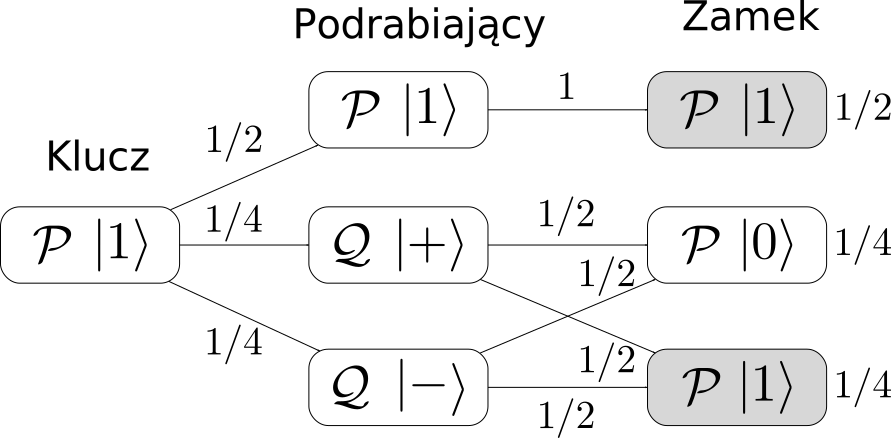
\includegraphics[width=0.7\textwidth]{pics/zamekkwantowy}
	\caption{Schemat obliczania prawdopodobieństwa prawidłowego
		zmierzenia stanu kubitu podrobionego klucza. Kolorem szarym oznaczono
		pomiary, które wykonuje zamek i~które zwrócą oczekiwany wynik.}
	\label{rys:zamek}
\end{figure}


Jak widać, nie jest łatwo podrobić klucze kwantowe. Czy~jednak istnieje
możliwość ich wykradzenia? Tego dowiemy się pod~koniec niniejszego rozdziału.

\section{Kwantowa dystrybucja klucza}
Wyobraźmy sobie, że~istnieją dwie osoby oddalone od~siebie fizycznie,
które chcą przesłać pomiędzy sobą pewną informację w~postaci ciągu
bitów. Informacja ta jest tajna i~nie powinna zostać przechwycona
przez~osoby trzecie\index{kwantowa dystrybucja klucza}. Powiedzmy, że
podmiotem nadającym informację jest Biblioteka Orbitalna Aleksandria
(zwana dalej Aleksandrią), odbierającym -- Centrum Komunikacji Kwantowej
(zwane dalej Centrum), a~osobą próbującą przechwycić informację -- Eve.

Klasyczne rozwiązanie tego problemu polega na~wykorzystaniu któregoś
z~algorytmów szyfrujących oraz~klasycznego kanału informacyjnego. Wadą tego
rozwiązania jest to, że~nie~mamy pewności, czy~algorytmy szyfrujące na~pewno są
bezpieczne. Nasza wiara w~ich bezpieczeństwo wynika tylko~i~wyłącznie
z~przekonania, że~nie~wiadomo, w~jaki sposób szybko i~efektywnie wykonywać pewne
algorytmy, takie jak~np.~algorytm znajdowania dzielników liczb.

\subsection{Szyfr Vernama}
Istnieje szyfr pozwalający przesyłać informację całkowicie bezpiecznie.
Jest to~szyfr Vernama\footnote{Od~nazwiska amerykańskiego inżyniera Gilberta Vernama
	(1890 -- 1960).}\index{szyfr Vernama}. Jego idea jest bardzo prosta.
Aleksandria i~Centrum
współdzielą pewien tylko sobie znany ciąg losowych bitów, czyli~klucz. Zakładamy,
że~Aleksandria chce przesłać tajną wiadomość w~postaci binarnej do~Centrum. Ażeby~ukryć
tę wiadomość przed~Eve, dla~każdego bitu wiadomości wykonuje operację XOR
z~odpowiednim bitem klucza. W~ten~sposób uzyskuje szyfrogram, który wysyła do~Centrum.
Po~otrzymaniu zaszyfrowanej wiadomości Centrum odwraca działanie Aleksandrii -- tzn.~wykonuje operację XOR na~każdym
bicie szyfrogramu z~odpowiednim bitem klucza, i~w~ten sposób odzyskuje oryginalną wiadomość
nadaną przez~Aleksandrię.

Operacja XOR działa na~dwóch bitach następująco: jeżeli~oba bity są różne, to
zwraca $1$, jeżeli~są równe -- to zwraca $0$.
Możemy zatem stworzyć Tabelę~\ref{tab:xor} wejść i~wyjść operacji XOR, w~której
dwie lewe kolumny odpowiadają argumentom operacji (wejściom), a~prawa kolumna
odpowiada wartościom (wyjściu).

\begin{table}[h!]
	\centering
	\begin{tabular}{ccc}
		$\text{we}_1$ & $\text{we}_2$ & $\text{wy}$ \\
		\toprule
		0             & 0             & 0           \\
		0             & 1             & 1           \\
		1             & 0             & 1           \\
		1             & 1             & 0
	\end{tabular}
	\caption{Tabela argumentów i~wartości operacji $\text{wy}=XOR(\text{we}_1, \text{we}_2)$}
	\label{tab:xor}
\end{table}

Oznaczmy zatem tajną wiadomość Aleksandrii jako ciąg bitów $$a_1, a_2, \ldots, a_n,$$
szyfrogram jako $$s_1, s_2, \ldots, s_n,$$ klucz jako $$k_1, k_2,
	\ldots, k_n,$$ a~wiadomość odczytaną przez~Centrum jako $$b_1, b_2, \ldots, b_n.$$
Wówczas w~procesie szyfrowania uzyskujemy szyfrogram ze~wzoru $s_i=XOR(a_i, k_i)$ dla~każdego
$i=1,2,\ldots,n$. Centrum natomiast deszyfruje wiadomość, korzystając ze~wzoru
$b_i=XOR(s_i, k_i)$. Łatwo można sprawdzić, że~dla~każdego $i=1,2,\ldots,n$ $a_i
	= b_i$, co oznacza, że~wiadomość otrzymana przez~Centrum jest tą, którą nadała Aleksandria.
Przykład takiego procesu szyfrowania i~deszyfrowania jest pokazany na~Rysunku~\ref{rys:vernam}.

\begin{figure}[h]
	\centering
	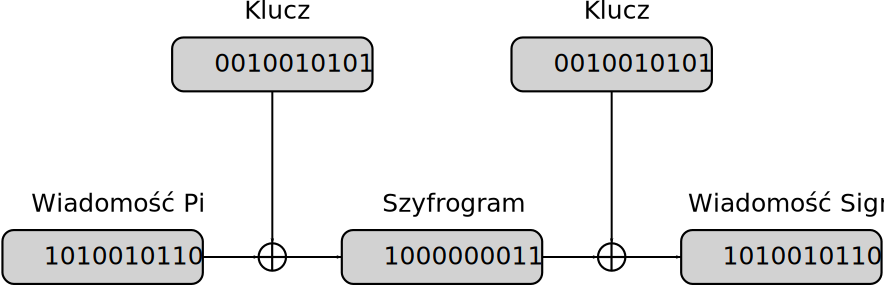
\includegraphics[width=0.7\linewidth]{pics/vernam}
	\caption{Przykład działania szyfru Vernama. Symbol $\oplus$ oznacza operację XOR.}
	\label{rys:vernam}
\end{figure}

Jeżeli~klucz jest całkowicie losowy, to~dla~Eve, która nie~zna klucza, szyfrogram
także jest całkowicie losowy i~nie~niesie żadnej informacji o~tajnej wiadomości.

\subsection{Protokół BB84}
Szyfr Vernama ma pewną wadę -- wymaga~on~tego, by~nadawca i~odbiorca wiadomości
korzystali z~klucza kryptograficznego, który ma długość samej wiadomości oraz~jest~całkowicie
losowy. Taki klucz -- po pierwsze -- trudno stworzyć, ponieważ nie~jest łatwo
wylosować całkowicie losowy ciąg bitów; a~po~drugie -- dystrybuować pomiędzy
nadawcę i~odbiorcę. Rozwiązaniem
problemu losowania i~dystrybucji klucza jest protokół
BB84\footnote{Zaproponowany w~roku 1984 przez Charlesa Bennetta i~Gilles'a
	Brassarda.}, który wykorzystuje kubity i~mechanikę kwantową
do~przygotowania i~dystrybucji klucza kryptograficznego.

Podobnie jak~w~konstrukcji zamków i~kluczy kwantowych, w~protokole BB84 używamy
czterech stanów jednokubitowych
$$
	\ket{0}, \ket{1}, \ket{+}=\frac{1}{\sqrt{2}}(\ket{0}+\ket{1})
	\text{ lub } \ket{-}=\frac{1}{\sqrt{2}}(\ket{0}-\ket{1})
$$
oraz~dwóch rodzajów pomiarów
$\mathcal{P}=\{\mat{P}_0=\ketbra{0}{0}, \mat{P}_1=\ketbra{1}{1}\}$ i
$\mathcal{Q}=\{\mat{Q}_+=\ketbra{+}{+}, \mat{Q}_-\ketbra{-}{-}\}$.

Aleksandria -- nadawca -- nadaje kubity w~stanach wymienionych powyżej, natomiast Centrum
-- odbiorca -- wykonuje wymienione powyżej pomiary. Zależność wyniku
pomiaru od~wysłanego stanu kubitu i~od~tego, jaki pomiar został na~nim dokonany, przedstawia
Tabela~\ref{tab:bb84}.

\begin{table}[h]
	\begin{center}
		\begin{tabular}{llc}
			stan      & pomiar        & wynik pomiaru                       \\
			\toprule
			$\ket{0}$ & $\mathcal{P}$ & $0$                                 \\
			\midrule
			$\ket{1}$ & $\mathcal{P}$ & $1$                                 \\
			\midrule
			$\ket{+}$ & $\mathcal{Q}$ & $+$                                 \\
			\midrule
			$\ket{-}$ & $\mathcal{Q}$ & $-$                                 \\
			\midrule
			$\ket{0}$ & $\mathcal{Q}$ & $+$ lub $-$ z $p_+=p_-=\frac{1}{2}$ \\
			\midrule
			$\ket{1}$ & $\mathcal{Q}$ & $+$ lub $-$ z $p_+=p_-=\frac{1}{2}$ \\
			\midrule
			$\ket{+}$ & $\mathcal{P}$ & $0$ lub $1$ z $p_0=p_1=\frac{1}{2}$ \\
			\midrule
			$\ket{-}$ & $\mathcal{P}$ & $0$ lub $1$ z $p_0=p_1=\frac{1}{2}$ \\
		\end{tabular}
		\caption{Zależność wyniku pomiaru od~stanu i~wybranego rodzaju pomiaru.}
		\label{tab:bb84}
	\end{center}
\end{table}

Jeżeli~stan nadawany przez~Aleksandrię nie~jest dopasowany do~pomiaru,
to wynik pomiaru tego stanu jest losowy, co~pokazują ostatnie cztery wiersze
tabeli. Dodatkowo po~pomiarze stan początkowy zmienia~się na~stan
odpowiadający wynikowi pomiaru. Fakt ten można wykorzystać do~wykrywania
podsłuchu podczas~przesyłania kubitów. Pozwala to na~stworzenie
protokołu dystrybucji kluczy kwantowych składającego~się z~poniższych
kroków:

\paragraph{Krok 1} Aleksandria wysyła sekwencję kubitów, z~których każdy jest w~losowo
i~niezależnie wybranym stanie: $\ket{0}$, $\ket{1}$,
$\ket{+}=\frac{\ket{0}+\ket{1}}{\sqrt{2}}$ lub~$\ket{-}=\frac{\ket{0}-\ket{1}}{\sqrt{2}}$.
\paragraph{Krok 2} Centrum dokonuje -- również losowo i~niezależnie --
wyboru, który z~dwóch pomiarów -- $\mathcal{P}$ lub~$\mathcal{Q}$ -- przeprowadzi na~każdym z~kubitów z~osobna.
\paragraph{Krok 3} Centrum zapisuje swój wybór i~wyniki pomiarów.
\paragraph{Krok 4} Centrum wysyła do~Aleksandrii w~sposób jawny swój wybór pomiarów.
\paragraph{Krok 5} Aleksandria przekazuje Centrum informację, które pomiary były dopasowane do stanów
nadanych kubitów.
\paragraph{Krok 6} Aleksandria i~Centrum dzielą kubity na~dwie części: jedna zawiera te, które
zostały zmierzone za~pomocą dopasowanego pomiaru, a~druga -- te, które nie~zostały zmierzone w~ten~sposób.

Możemy zauważyć, że~średnio w~połowie przypadków został użyty
niedopasowany pomiar. Przypadki te muszą zostać odrzucone, gdyż~wynik
niedopasowanego pomiaru jest całkowicie losowy.

Jeżeli~nie~zaistniały przekłamania i~nikt nie~ingerował w~proces
transmisji, to ok.~50\% kubitów zmierzonych przez~Centrum ma ten sam  stan, który został nadany w~Kroku 1 przez Aleksandrię. Te właśnie kubity można wykorzystać do~stworzenia klucza kryptograficznego.

\paragraph{Krok 7} Aleksandria i~Centrum wybierają pewien wspólny
podzbiór kubitów spośród tych, które zostały zmierzone przy~użyciu
dopasowanego pomiaru, i~w~sposób jawny je porównują. Kubity te oczywiście
będzie trzeba odrzucić, jako że~zostały ujawnione.

Jeżeli~nie~doszło do~podsłuchania transmisji kubitów, to porównanie
powinno dać całkowicie zgodne wyniki. Wówczas Aleksandria i~Centrum
przypisują stanom $\ket{0}$, $\ket{-}$ bit $0$, a~stanom $\ket{1}$,
$\ket{+}$ bit $1$. Zatem teraz Aleksandria i~Centrum mają wspólny
losowy klucz kryptograficzny, którego mogą użyć do~przekazania sobie
zaszyfrowanej szyfrem Vernama wiadomości.

Jeżeli~podczas wykonywania protokołu Aleksandria i~Centrum wykryły
jakiekolwiek niezgodności, oznacza to, że~kubity zostały już~poddane
pomiarowi przez~osobę trzecią i~nie~należy ich używać do~tworzenia
klucza. W~takim przypadku muszą zaniechać przesyłania tajnej informacji.

Zastanówmy~się, jakie próby ataku może podjąć Eve. Nie~może skopiować
stanu kubitu i~zmierzyć jego kopii, gdyż~tego zabrania twierdzenie
o~zakazie klonowania. Może natomiast wpiąć~się do~kwantowego kanału
transmisji i~przechwytywać wszystkie kubity nadesłane przez~Aleksandrię,
dokonywać na~nich pomiaru i~następnie odsyłać do~Centrum. Taka technika
podsłuchu jest bardzo łatwa do~zdemaskowania, ponieważ skoro Eve nie wie, jakie
kubity zostały nadane, nie~wie też, jaki pomiar powinna wybrać. Jeśli więc Eve wybierze
niewłaściwy pomiar, doprowadzi do~zmiany stanów kubitów, co --
po~wymianie klucza -- Aleksandria i~Centrum z~łatwością wykryją. Eve
może również przechwytywać tylko niektóre kubity i~je mierzyć, ale~wtedy
nie~uzyska całego klucza kryptograficznego, a~jej działanie też~może
zostać wykryte.

Tabela~\ref{tab:bb84przyklad} pokazuje, jak może przebiegać krótki
proces ustalania klucza przez Aleksandrię i~Centrum, gdy~Eve
nie~podsłuchuje. Natomiast w~Tabeli~\ref{tab:bb84przykladzewą} pokazano,
co się~dzieje, gdy~Eve podsłuchuje komunikację kwantową.

\definecolor{Gray}{gray}{0.9}
\def\colw{0.7em}
\newcolumntype{P}[1]{>{\centering\arraybackslash}p{#1}}
\newcolumntype{g}{>{\columncolor{Gray}}P{\colw}}
\newcolumntype{w}{P{\colw}}
\begin{table}[h]
	\resizebox{\textwidth}{!}{
		\centering
		\tiny
		\begin{tabular}{l|gggwwwgwgwwgwgwwwggg}
			$A_1$ & $\ket{0}$     & $\ket{1}$     & $\ket{1}$     & $\ket{+}$     & $\ket{1}$     & $\ket{+}$     & $\ket{+}$     & $\ket{-}$     & $\ket{-}$     & $\ket{0}$     & $\ket{0}$     & $\ket{-}$     & $\ket{-}$     & $\ket{1}$     & $\ket{0}$     & $\ket{1}$     & $\ket{+}$     & $\ket{1}$     & $\ket{0}$     & $\ket{0}$     \\
			$C_1$ & $\mathcal{P}$ & $\mathcal{P}$ & $\mathcal{P}$ & $\mathcal{P}$ & $\mathcal{Q}$ & $\mathcal{P}$ & $\mathcal{Q}$ & $\mathcal{P}$ & $\mathcal{Q}$ & $\mathcal{Q}$ & $\mathcal{Q}$ & $\mathcal{Q}$ & $\mathcal{P}$ & $\mathcal{P}$ & $\mathcal{Q}$ & $\mathcal{Q}$ & $\mathcal{P}$ & $\mathcal{P}$ & $\mathcal{P}$ & $\mathcal{P}$ \\
			$C_2$ & $\ket{0}$     & $\ket{1}$     & $\ket{1}$     & $\ket{1}$     & $\ket{-}$     & $\ket{0}$     & $\ket{+}$     & $\ket{0}$     & $\ket{-}$     & $\ket{+}$     & $\ket{-}$     & $\ket{-}$     & $\ket{1}$     & $\ket{1}$     & $\ket{-}$     & $\ket{-}$     & $\ket{0}$     & $\ket{1}$     & $\ket{0}$     & $\ket{0}$     \\
			bit   & 0             & 1             & 1             &               &               &               & 1             &               & 0             &               &               & 0             &               & 1             &               &               &               & 1             & 0             & 0
		\end{tabular}
	}
	\caption{Przykład realizacji protokołu BB84 bez~podsłuchu. Oznaczenia wierszy:
		$A_1$ -- stany wysłane przez~Aleksandrię,
		$C_1$ -- pomiary wybrane przez~Centrum,
		$C_2$ -- stany po~pomiarze Centrum,
		bit -- bit klucza.
		Kolumny oznaczone na~szaro wyróżniają przypadki, dla~których stan kubitu
		nadanego przez~Aleksandrię pokrywa~się z~kubitem zmierzonym przez~Centrum. We~wszystkich
		przypadkach, w~których Aleksandria nadała kubit w~stanie dopasowanym do~pomiaru Centrum, Centrum zmierzyło
		odpowiedni stan -- zatem Aleksandria i~Centrum nie~mają powodu podejrzewać, że~ktoś podsłuchiwał
		ustalanie klucza.
	}
	\label{tab:bb84przyklad}
\end{table}

\begin{table}[h]
	\resizebox{\textwidth}{!}{
		\centering\tiny
		\begin{tabular}{l|wwwwgwwgwwwwgwwgwwww}
			$A_1$ & $\ket{0}$     & $\ket{1}$     & $\ket{1}$     & $\ket{+}$     & $\ket{1}$     & $\ket{+}$     & $\ket{+}$     & $\ket{-}$     & $\ket{-}$     & $\ket{0}$     & $\ket{0}$     & $\ket{-}$     & $\ket{-}$     & $\ket{1}$     & $\ket{0}$     & $\ket{1}$     & $\ket{+}$     & $\ket{1}$     & $\ket{0}$     & $\ket{0}$     \\
			$E_1$ & $\mathcal{P}$ & $\mathcal{P}$ & $\mathcal{Q}$ & $\mathcal{P}$ & $\mathcal{Q}$ & $\mathcal{P}$ & $\mathcal{Q}$ & $\mathcal{P}$ & $\mathcal{Q}$ & $\mathcal{Q}$ & $\mathcal{Q}$ & $\mathcal{Q}$ & $\mathcal{P}$ & $\mathcal{P}$ & $\mathcal{Q}$ & $\mathcal{Q}$ & $\mathcal{P}$ & $\mathcal{P}$ & $\mathcal{P}$ & $\mathcal{P}$ \\
			$E_2$ & $\ket{0}$     & $\ket{1}$     & $\ket{+}$     & $\ket{1}$     & $\ket{-}$     & $\ket{0}$     & $\ket{+}$     & $\ket{0}$     & $\ket{-}$     & $\ket{+}$     & $\ket{-}$     & $\ket{-}$     & $\ket{1}$     & $\ket{1}$     & $\ket{-}$     & $\ket{-}$     & $\ket{0}$     & $\ket{1}$     & $\ket{0}$     & $\ket{0}$     \\
			$C_1$ & $\mathcal{Q}$ & $\mathcal{P}$ & $\mathcal{P}$ & $\mathcal{P}$ & $\mathcal{P}$ & $\mathcal{P}$ & $\mathcal{Q}$ & $\mathcal{Q}$ & $\mathcal{Q}$ & $\mathcal{Q}$ & $\mathcal{Q}$ & $\mathcal{Q}$ & $\mathcal{Q}$ & $\mathcal{P}$ & $\mathcal{Q}$ & $\mathcal{P}$ & $\mathcal{P}$ & $\mathcal{P}$ & $\mathcal{Q}$ & $\mathcal{Q}$ \\
			$C_2$ & $\ket{+}$     & $\ket{1}$     & $\ket{1}$     & $\ket{1}$     & $\ket{0}$     & $\ket{0}$     & $\ket{+}$     & $\ket{+}$     & $\ket{-}$     & $\ket{+}$     & $\ket{-}$     & $\ket{-}$     & $\ket{+}$     & $\ket{1}$     & $\ket{-}$     & $\ket{0}$     & $\ket{0}$     & $\ket{1}$     & $\ket{+}$     & $\ket{+}$
		\end{tabular}
	}
	\caption{
		Przykład realizacji protokołu BB84 z~podsłuchem. Oznaczenia wierszy:
		$A_1$ -- stany wysłane przez~Aleksandrię,
		$E_1$ -- pomiary wybrane przez~Eve,
		$E_2$ -- stany po~pomiarze Eve,
		$C_1$ -- pomiary wybrane przez~Centrum,
		$C_2$ -- stany po~pomiarze Centrum.
		Kolumny oznaczone na~szaro wyróżniają przypadki, dla~których stan kubitu
		nadanego przez~Aleksandrię nie~pokrywa~się z~kubitem zmierzonym przez~Centrum. Te przypadki wskazują Aleksandrii i~Centrum, że~mogło dojść do~podsłuchu.
	}
	\label{tab:bb84przykladzewą}
\end{table}

Bezpieczeństwo protokołu BB84 zależy od~naszej ufności w~skuteczność
mechaniki kwantowej -- najlepiej potwierdzonej współczesnej teorii
fizycznej -- w~przeciwieństwie do~klasycznych protokołów kryptografii
asymetrycznej, w~przypadku której musimy zakładać, że~nikt nie~zna
skutecznych metod faktoryzacji liczb lub~liczenia logarytmu dyskretnego.

\section{Teleportacja kwantowa}
Rozważmy trzy osoby\footnote{Zwykle w protokole teleportacji myślimy o
	dwóch osobach -- jednej z dwoma kubitami, która chce przesłać informację,
	i drugiej z jednym kubitem, która jest odbiorcą.} -- Bretta, Eve i
Roberta. Każde z nich ma do dyspozycji jeden kubit. Wyobraźmy sobie, że
kubit~Bretta jest w nieznanym stanie, a Eve chce przesłać stan kubitu
Bretta do Roberta. Eve może zbliżyć swój kubit do kubitu Bretta, jednak
nie~ma możliwości przesłania do~Roberta informacji kwantowej --
tzn.~stanów kwantowych. Może do~niego natomiast przesłać informację
klasyczną. Jeśli~ma~do~dyspozycji tylko jedną kopię stanu, jest to oczywiście
niemożliwe. Natomiast jeżeli~Eve i~Robert współdzielą splątany stan
Bella, to staje~się możliwe przesłanie informacji klasycznej. Taki
proces przesyłania stanu kwantowego z~wykorzystaniem stanu splątanego
nazywamy protokołem \newterm{teleportacji kwantowej}\index{teleportacja
	kwantowa}. Schematyczna ilustracja tego protokołu jest przedstawiona
na~Rysunku~\ref{rys:teleportacja}. Pierwszy kubit to kubit Bretta, drugi należy do Eve, natomiast trzeci kubit ma
Robert. Pierwszy kubit jest w~stanie, który Eve chce przesłać Robertowi,
natomiast drugi i~trzeci kubit są w~stanie Bella
$\ket{\Phi^+}=\frac{1}{\sqrt{2}}(\ket{00}+\ket{11})$.

\begin{figure}[h]
	\centering
	\includegraphics[width=0.8\textwidth]{pics/teleportation} \caption{Obwód
		teleportacji kwantowej. Linie poziome oznaczają kubity. Pionowa linia
		zygzakowata oznacza stan splątany. Linie podwójne oznaczają klasyczne bity.
		Pozioma linia przerywana oddziela układy Bretta i Alice od~układu Roberta.}
	\label{rys:teleportacja}
\end{figure}


Ponieważ nie~wiemy nic o~stanie kubitu Bretta, zapiszmy go w~ogólnej postaci
$$
	\ket{\psi} = \alpha \ket{0} + \beta \ket{1}.
$$
Wówczas stan początkowy układu jest następujący:
\begin{equation*}
	\begin{split}
		\ket{\psi_{t=0}} &=  \ket{\psi} \otimes \ket{\Phi^+}  =\\
		&= \ket{\psi} \otimes \frac{1}{\sqrt{2}}\left( \ket{0} \otimes \ket{0} +\ket{1} \otimes \ket{1} \right) = \\
		&= \left(\alpha \ket{0} + \beta  \ket{1}\right) \otimes \frac{1}{\sqrt{2}}\left( \ket{0} \otimes \ket{0} +\ket{1} \otimes \ket{1} \right)= \\
		&= \frac{1}{\sqrt{2}} \left(\alpha \ket{000} + \alpha \ket{011} + \beta  \ket{100} + \beta  \ket{111}  \right).
	\end{split}
\end{equation*}
Eve nakłada teraz bramkę~$\mat{CNOT}_1^2$ na~kubity swój i
Bretta\footnote{Jest to możliwe, jeśli zakładamy, że Eve może zbliżyć swój
	kubit do kubitu Bretta i~nakładać bramki jedno- i dwukubitowe na oba
	kubity.}, a~stan układu zmienia~się na~:
\begin{equation*}
	\begin{split}
		\ket{\psi_{t=1}} &= (\mat{CNOT}_1^2\otimes \mat{\id}) \frac{1}{\sqrt{2}} \left(\alpha \ket{000} + \alpha \ket{011} + \beta \ket{100} + \beta \ket{111}  \right) =\\
		&=\frac{1}{\sqrt{2}} \left(\alpha \ket{000} + \alpha \ket{011} + \beta \ket{110} + \beta \ket{101}  \right).
	\end{split}
\end{equation*}
Następnie Eve nakłada bramkę Hadamarda na~kubit Bretta, i~w~ten sposób zmienia stan na:
\begin{equation*}
	\begin{split}
		\ket{\psi_{t=2}} &=( \mat{H}\otimes\mat{\id}\otimes\mat{\id}) \frac{1}{\sqrt{2}} \left(\alpha \ket{000} + \alpha \ket{011} + \beta \ket{110} + \beta \ket{101}  \right) =\\
		&= \frac{1}{\sqrt{2}} \Big(
		\alpha \frac{1}{\sqrt{2}}(\ket{0}+\ket{1})\otimes (\ket{00} +  \ket{11}) + \\
		& + \beta \frac{1}{\sqrt{2}}(\ket{0}-\ket{1})\otimes(\ket{10} + \ket{01}) \Big) =\\
		&= \frac{1}{2} (\alpha \ket{000} + \alpha \ket{100}  + \alpha \ket{011} + \alpha \ket{111} + \\
		&+ \beta \ket{010} + \beta \ket{001} - \beta \ket{110} - \beta \ket{101} ).
	\end{split}
\end{equation*}
Następnie Eve mierzy pierwsze dwa kubity przy~użyciu pomiaru częściowego $\mathcal{P}$ składającego~się z~macierzy
\begin{equation*}
	\begin{split}
		\mathcal{P} = \{&\mat{P}_{00?}=\ketbra{0}{0}\otimes\ketbra{0}{0}\otimes\mat{\id}, \mat{P}_{01?}=\ketbra{0}{0}\otimes\ketbra{1}{1}\otimes\mat{\id}, \\
		&\mat{P}_{10?}=\ketbra{1}{1}\otimes\ketbra{0}{0}\otimes\mat{\id}, \mat{P}_{11?}=\ketbra{1}{1}\otimes\ketbra{1}{1}\otimes\mat{\id}\}
	\end{split}
\end{equation*}
i~otrzymuje -- w~zależności od~wyniku pomiaru -- z~jednakowym prawdopodobieństwem stany:
\begin{itemize}
	\item dla wyniku $00?$: $$\frac{1}{\sqrt{2}}\left(\alpha \ket{000}  + \beta \ket{001}\right) = \frac{1}{\sqrt{2}}\left(\ket{00}\otimes \ket{\psi}\right),$$
	\item dla wyniku $01?$: $$\frac{1}{\sqrt{2}}\left(\alpha \ket{011}  + \beta \ket{010}\right) = \frac{1}{\sqrt{2}}\left(\ket{01}\otimes \mat{Z}\ket{\psi}\right),$$
	\item dla wyniku $10?$: $$\frac{1}{\sqrt{2}}\left(\alpha \ket{100}  - \beta \ket{101}\right) = \frac{1}{\sqrt{2}}\left(\ket{10}\otimes \mat{X}\ket{\psi}\right),$$
	\item dla wyniku $11?$: $$\frac{1}{\sqrt{2}}\left(\alpha \ket{111}  - \beta \ket{110}\right) = \frac{1}{\sqrt{2}}\left(\ket{11}\otimes \mat{X}\mat{Z}\ket{\psi}\right).$$
\end{itemize}

Zauważmy, że~w~zależności od~wyniku pomiaru Eve stan kubitu Roberta jest
w tym momencie jednym z~czterech stanów: $\ket{\psi}$,
$\mat{Z}\ket{\psi}$, $\mat{X}\ket{\psi}$ lub~$\mat{X}\mat{Z}\ket{\psi}$.
Widać zatem, że~jeżeli~Robert wie, jaki wynik uzyskuje Eve, może~--
przy~użyciu kombinacji bramek $\mat{X}$ i~$\mat{Z}$ -- zmienić swój stan
tak, by~odzyskać oryginalny stan Bretta. W~przypadku wyniku pomiaru $00$
nie~musi robić nic; w~przypadku $01$ nakłada na~swój kubit bramkę
odwrotną do~$\mat{X}$, czyli~$\mat{X}^\dagger$; w~przypadku $10$ nakłada
bramkę $\mat{Z}^\dagger$, a~w~przypadku wyniku pomiaru $11$ -- bramki
$\mat{Z}^\dagger \mat{X}^\dagger$.

Zatem jeśli wykorzysta się splątanie kwantowe oraz~informację klasyczną, można
przenieść stan kubitu Bretta na~kubit Roberta, co może pozwolić
np.~na~kradzież kluczy do~zamków kwantowych, które opisywaliśmy
wcześniej. Na końcu tego rozdziału wyjaśnione jest jak doszło do kradzieży
klucza w komiksie.
